\documentclass{aptpub}
\usepackage{graphicx}
\usepackage{bookmark}
\authornames{AUTHOR NAMES} % insert the authors here for use in running head. If three or more authors please use (for example) M.~YARROW {\it et al}. Author names should follow the same M.~YARROW format and if two authors, separate by 'AND'.
\shorttitle{Short title} % insert short title here for use in running head

% Put any of your own definitions here.

%\numberwithin{equation}{section}  % If you number theorems, etc. within sections,
                                   % then please uncomment this line to number
                                   % equations with sections too.
\def\E{\mathbb{E}}
\def\R{\mathbb{R}}
\begin{document}%\recd{}{}%Do not alter this line.

\title{Title} % insert title - use \\ if it requires more than one line.

\authorone[Affiliation]{Author name} 
%Affiliation is just the name of your university or institution, for example 'University of Sheffield'. Author names should be of the form 'Mark Yarrow'. 
%Authors should be ordered alphabetically subject to the convention in that particular authors country. For example 'Remco van der Hofstad' would be listed under 'H' as is standard in the Netherlands. 


%Please use the following format for addresses and emails. The APT office will sort this out after you submit your files.
\addressone{Full address} % Your postal address goes here.
\emailone{Full email address} %Authors email goes here.

\begin{abstract}
% text of abstract goes here!
\end{abstract}

\keywords{}%insert keywords separated by a semicolon. You should avoid including keywords which also appear in the title.

\ams{}{}% insert the primary 2020 Maths Subject Classification number in the first bracket
		% and the secondary ams number(s) in the second bracket
		% e.g. \ams{60E20}{49G03;49F10}
		%Maximum of three in each, ideally one or two in each primary and secondary.
		%codes found here ``https://mathscinet.ams.org/msnhtml/msc2020.pdf''


\section{Introduction} % Initial capital letter, then lower case. No full stop.

% Write the text of your paper using normal LaTeX commands.
% For instance, you can use the `\cite' command~\cite{ref1}.
% When giving citations a numbering system is preferred~\cite{ref2},
% but an author--date system is also acceptable~\cite{ref3}.

%\subsection{Introduction} % Initial capital letter, then lower case. No full stop.
Let $X_1, X_2, \dots, X_N$ be i.i.d. sampled from a spherical symmetric distribution in $\mathbb{R}^d$.
The convex hull $H_N$ of these $N$ points are an interrupted research topic in stochastic and integral geometry
\cite{schneider2008stochastic}.
The main aim of this paper is to provide a integral formula for $\E[F_N]$, the expected value of the number of $d-1$ dimensional hyperplanes
of $H_N$,
and derive its asymptotic expression
for three kinds of distribution families. Furthermore, the estimation of $\E[F_N]$ is used to obtain the upper bound
of the probability $p_{n,d}$, another sample falls outside of the random convex hull. This probability can be used to
measure the interpolation ability of training data in machine learning
\cite{balestriero2021learning}.

The asymptotic expression of $\E[F_N]$ as $N\to \infty$
was studied firstly by R{\'e}nyi \cite{renyi1963konvexe}.
In his paper the distribution considered
is 2D standard gaussian or uniform distribution within a convex region with continuous curvature.
Later on, Carnal \cite{carnal1970konvexe} generalized R{\'e}nyi's work,
and studied general symmetric distribution in 2d,
and obtained the asymptotic expression of $\E[F_N]$
in three different distribution families.

For $d>2$, the breakthrough is made firstly by
Raynaud
\cite{raynaud1970enveloppe}.
He obtains the asymptotic formula for uniform distribution within a hyperball
and standard gaussian in $\mathbb{R}^d$.
Then Dwyer \cite{dwyer1991convex} obtains the order of $\E[F_N]$ about $N$
in three different distribution families.

However, the asymptotic formula of $\E[F_N]$ is generally unknown.
In our work, we obtain this formula by generalizing the Carnal's integral formula
of $H(x)=P(d_{12}\geq x)$ to higher dimensions in Section \ref{sec:int_f}.
Then we obtain the asymptotic
expression for $\E[F_N]$ in three different distribution families in Section \ref{sec:three_distriutions}.
Based on this result,
we discuss the condition when $p_{n,d}$ converges to zero as $N,d \to \infty$
in Section \ref{sec:sample_complexity}.
This condition is applied to explain some dimension explosion problems
in the field of machine learning.

Without specific mention, the $d$-dimensional distribution considered in this paper is spherically symmetric.
Below we define some notations which are to be used throughout this paper.
Let $F(x)=P(|X|\geq x)$ represents the probability that a random point lies outside
a d-sphere. $G(x)=P(X_1\geq x)$ is the one dimensional marginal distribution.
Let $d$ represents the distance from the origin to the random hyperplane, spanned by $X_1, \dots, X_d$.
In 2d, $d=d_{12}$, the distance to the random line passing $X_1, X_2$. $H(x)=P(d\geq x)$ is
the probability outside of the random hyperplane.
\section{Integral formula}\label{sec:int_f}
In 2d, the integral formula for $\E[F_N]$ is given as
\begin{align}
     \E[F_N] &= \binom{N}{2} \int_0^{+\infty} 
     \left[G(x)^{N-2} + (1-G(x))^{N-2} \right]|dH(x)| 
     \label{eq:E_F_N_2_d}
\end{align}
The integral formula of $\E[F_N]$ involves the function $G(x)$ and $H(x)$,
both of which can be expressed in term of $F(x)$:
\begin{align}
   G(x) &=\frac{1}{\pi} \arccos\frac{x}{y} |dF(y)| \\
     H(x) &= \frac{2}{\pi} \int_x^{\infty} \arccos \frac{x}{z} |d(F^2(z))|
     \label{eq:H_expression_2_dim}
\end{align}
For $d\geq 2$, the integral formula is generalized as
\begin{align}
     \E[F_N] &= \binom{N}{d} \int_0^{+\infty} 
     \left[G(x)^{N-d} + (1-G(x))^{N-d} \right]|dH(x)| 
     \label{eq:E_F_N_d}
\end{align}
Formula first appeared in the proof section of \cite{raynaud1970enveloppe}
and can further to generalized to contain other integrands \cite{barany2008random}.
Dwyer obtains the integral formula for $G(x)$ in $d\geq 2$ as:
\begin{align}\label{eq:G_d_kappa}
     G(x) & = \int_x^{+\infty} \kappa(\frac{x}{y}) |dF(y)|
\end{align}
where $\kappa(r)$ is the fraction of the surface area of a unit d-sphere
cut off by a plane at distance $r$ from the origin.

Our main theorem gives the integral formula for $H(x)$ in $d\geq 2$:
\begin{theorem}\label{thm:H}
Define the auxiliary function $\kappa(x,y)$ and $K(x)$ as follows: 
     \begin{align}
          \lambda_d(r) & :=(1-r^2)^{\frac{d-2}{2}}
          \label{eq:lambda_r}\\
          K(x) &:=P(\sqrt{X_1^2+X_2^2}>x)=
          \int_x^{+\infty}
          \lambda_d \left(\frac{x}{y} \right)|dF(y)|
          \label{eq:K_x}
      \end{align}
Then
\begin{equation}
     H(x) = \frac{2}{\pi}
     \int_x^{+\infty} \arccos\frac{x}{y}
     |d K^d(y)|\label{eq:H_expression_d_dim}
\end{equation}
\end{theorem}
It is easy to observe that \eqref{eq:H_expression_d_dim} reduces to 
\eqref{eq:H_expression_2_dim} when $d=2$.
For standard Gaussian distributions, $X_1, X_2$ are independent 1d
Gaussian, therefore $K(x) = e^{-x^2/2}$. In fact, $1-K(x)$ is the CDF of Rayleigh distribution.
%For general spherical distributions, the function $K(x)$ itself is irreverent with the dimension $d$.
The detailed proof of Theorem \ref{thm:H}
is provided in Appendix \ref{app:th}.

\section{Three distribution families}\label{sec:three_distriutions}
Notice that in \eqref{eq:E_F_N_2_d}, as $G(x)<\frac{1}{2}$ for $x>0$, the integration containing the
term $G(x)^{N-2}$ decays exponentially fast as $N\to \infty$.
\subsection{Distributions with algebraic tails}
\subsection{Distributions with exponential tails}
\subsection{Distributions with truncated tails}
\section{Sample complexity in data interpolation}\label{sec:sample_complexity}
% If you write a theorem, lemma, proposition etc please use the
% appropriate environments. For instance:

%Use {rem} for a Remark, {rems} for Remarks, {defn}
                                  %for a definition, etc. numbered within sections.

                                  %If numbering theorems, etc. within sections,
                                  %uncomment the line in the preamble to number
                                  %equations within sections too.
     %For unnumbered Remarks, use {remnn}, {defnn}, etc.

% The proof of a result should go in the proof environment:

%If your paper includes appendices, then precede the first of them by the command
\appendix
%and then carry on using the \section and \subsection commands, as above.

\section{Proof of Theorem \ref{thm:H}}\label{app:th}
\begin{lemma}\label{lem:F_0}
     Let $F_0$ represent the
probability that the distance from the origin to the straight line
$X_1X_2$ is larger than $x$. Then 
\begin{equation}\label{eq:F_0_expression}
     F_0(x)=\frac{2\Gamma(\frac{d}{2})}
     {\sqrt{\pi}\Gamma(\frac{d-1}{2})}
     \int_x^{\infty} |dF(y)|
     \int_x^{y} |dF(z)| \int_{a_2/z}^{a_1 /z} (1-u^2)^{\frac{d-3}{2}}du
 \end{equation}
where
\begin{align}
     a_1 & =\frac{x^2}{y}+\sqrt{z^2-x^2}\sqrt{1-\frac{x^2}{y^2}} > 0
     \label{eq:a_1} \\
a_2 & =\frac{x^2}{y}-\sqrt{z^2-x^2}\sqrt{1-\frac{x^2}{y^2}} < 0
\label{eq:a_2}
\end{align}
\end{lemma}
Lemma gives the integral formula for $P(d_{12}\geq x)$ in $\R^d$.
The geometric meaning of $a_1, |a_2|$ is illustrated in Figure
\ref{fig:a1a2}. That is, if we assume
\begin{equation}\label{eq:theta_1_theta_2}
     \cos\theta_1=\frac{x}{z},
     \textrm{ and } \cos\theta_2=\frac{x}{y} 
\end{equation}
then
\begin{equation}\label{eq:a_1_a_2}
     \frac{a_1}{z} = \cos(\theta_2 - \theta_1),
     \quad
     \frac{a_2}{z} = \cos(\theta_2+\theta_1)           
\end{equation}

\begin{figure}[!ht]
     \centering
     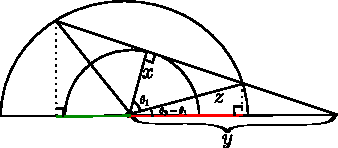
\includegraphics[width=0.8\textwidth]{dessin.pdf}
     \caption{The red line represents $a_1$ while the green line is the length of $|a_2|$.}
     \label{fig:a1a2}
\end{figure}
When $d=2$, using $\int \frac{dx}{\sqrt{1-x^2}} = -\arccos x + C$,
we obtain
$$
F_0(x)=\frac{4}{\pi} \int_x^{\infty} \arccos\frac{x}{z}|dF(y)|
\int_x^{y} |dF(z)|dz
$$
which reduces to \eqref{eq:H_expression_2_dim}.
\begin{proof}[Proof of Lemma \ref{lem:F_0}]
For $d\geq 2$ and $x<z<y$, we follow the geometric approach adopted to derive
$H(x)$ in \cite{carnal1970konvexe}.
Then we only need to compute the ratio of surface area
on the sphere with radius $z$. This is the area between
two planes at distance $\frac{a_1}{z}$ and $\frac{a_2}{z}$
on a unit sphere. From (1.1) of \cite{dwyer1991convex},
this ratio equals $\kappa(\frac{a_2}{z}) - \kappa(\frac{a_1}{z})$
where
\begin{equation}
     \kappa(r) = \frac{\Gamma(\frac{d}{2})}
     {\sqrt{\pi}\Gamma(\frac{d-1}{2})}\int_r^{1}
     (1-u^2)^{(d-3)/2}du
\end{equation}
Notice that $\kappa$ has been used in \eqref{eq:G_d_kappa}.
\end{proof}
To show 
$K(x) = \int_x^{+\infty} \lambda_d(\frac{x}{y})|dF(y)|$
in \eqref{eq:K_x},
we only need to connect $\lambda_d(r)$ with its geometric meaning,
which is given in the following lemma:
\begin{lemma}
     The ratio of surface area of a unit d-sphere,
     satisfying $x_1^2+x_2^2\geq r$ is $\lambda_d(r)$,
     defined in \eqref{eq:lambda_r}.
\end{lemma}
\begin{proof}
     Following \cite{dwyer1991convex}, we use $\kappa_d = 2\pi^{d/2}/\Gamma(d/2)$
     to represent the surface area of the unit d-sphere. Then
     \begin{align}
          \lambda_d(r) &=\frac{1}{\kappa_d} 
          \cdot 2\int_{\substack{x_1^2+x_2^2\geq r^2\\
          x_1^2+\dots+x_{d-1}^2\leq 1 }} 
          \frac{1}{\sqrt{1-x_1^2-\dots -x_{d-1}^2}} dx_1 \dots dx_{d-1}\\
      &= \frac{4\pi}{\kappa_d} \int_r^1 xdx \int_{x_3^2+\dots + x_{d-1}^2 \leq 1-x^2} \frac{dx_3\dots dx_{d-1}}
      {\sqrt{1-x^2-x_3^2-\dots -x_{d-1}^2}} \\
      &=\frac{4\pi \kappa_{d-3}}{\kappa_d} \int_r^1 xdx \int_0^{\sqrt{1-x^2}} \frac{y^{d-4}dy}{\sqrt{1-x^2-y^2}}\\
      &=\frac{4\pi \kappa_{d-3}}{\kappa_d} \int_0^{\sqrt{1-r^2}} y^{d-4}dy \int_r^{\sqrt{1-y^2}} \frac{xdx}{\sqrt{1-x^2-y^2}}\\
      &=\frac{4\pi \kappa_{d-3}}{\kappa_d} \int_0^{\sqrt{1-r^2}} y^{d-4}\sqrt{1-r^2-y^2} dy\\
      &=\frac{4\pi \kappa_{d-3}}{\kappa_d}  \frac{B(\frac{3}{2 }, \frac{d-3}{2})}{2}(1-r^2)^{(d-2)/2}\\
      &=  (1-r^2)^{(d-2)/2}
      \end{align}
\end{proof}

\begin{lemma}\label{lem:cn_integration}
For $0<c<1$ and $n$ is a non-negative positive integer,   
\begin{equation}
    \int_0^{c}
    [\frac{1}{(1-t)^{n+1}}+\frac{1}{(1+t)^{n+1}}]
    (c^2- t^2)^{(n-1)/2}dt
    =B(\frac{n+1}{2}, \frac{1}{2})
    \frac{c^n}{(1-c^2)^{(n+1)/2}}
    \end{equation}\label{eq:c_int_eq}
\end{lemma}
\begin{proof}[Proof of Lemma \ref{lem:cn_integration}]
     When $n=0$, the left hand side equals
     \begin{align*}
          \int_0^c \frac{2}{(1-t^2)\sqrt{c^2-t^2}} dt
          = \int_0^{\sqrt{c}} \frac{1}{(1-t) \sqrt{t} \sqrt{c^2-t} }dt
     \end{align*}     
     We make change of variables $x=\sqrt{t/(c^2-t)}$ and obtain
     the value $\frac{\pi}{(1-c^2)^{1/2}}$, which equals
     the right hand side.
     When $n=1$, we can use integration
     to show \eqref{eq:c_int_eq} holds.

     Let
\begin{equation}\label{eq:f_n_c_def}
h(n,c)=   \int_0^{c}
    [\frac{1}{(1-t)^{n+1}}+\frac{1}{(1+t)^{n+1}}]
    (c^2- t^2)^{(n-1)/2}dt
\end{equation}
When $n\geq 2$, by integration by parts 
we have 
\begin{equation}\label{eq:tmp_n_u_d_f_n}
    \frac{n}{n-1}h(n,c)
    =\int_0^{c}
    \left[\frac{1}{(1-t)^{n}}
    -\frac{1}{(1+t)^{n}}
    \right]
    t(c^2- t^2)^{(n-3)/2}
    dt
\end{equation}
Let $t=\frac{(1+t)-(1-t)}{2}$ in the right hand side
of \eqref{eq:tmp_n_u_d_f_n}, then
\begin{equation}
    2\frac{n}{n-1}h(n,c)
=    -h(n-2,c)  
+ \int_0^{c}
\left[\frac{1+t}{(1-t)^{n}}
+\frac{1-t}{(1+t)^{n}}
\right]
(c^2- t^2)^{(n-3)/2}
dt
\end{equation}
On the other hand,
From \eqref{eq:f_n_c_def},
$(c^2-t^2)^{(n-1)/2}
=[(c^2-1)+(1-t^2)](c^2-t^2)^{(n-3)/2}$
\begin{equation}
    f(n, c) = \frac{c^2-1}{2c}\frac{2}{n-1}\frac{\partial h(n,c)}{\partial c}
    +  \int_0^{c}
    \left[\frac{1+t}{(1-t)^{n}}
    +\frac{1-t}{(1+t)^{n}}
    \right]
    (c^2- t^2)^{(n-3)/2}
    dt
\end{equation}
Therefore,
\begin{equation}\label{eq:sim_1tc}
    h(n,c)=\frac{c^2-1}{2c}\frac{2}{n-1}\frac{\partial h(n,c)}{\partial c}
    + [2\frac{n}{n-1} h(n,c) + h(n-2, c)]
\end{equation}
then we can use induction and solve this
first order linear ODE about $h(n,c)$.
With initial condition $h(n,0)=0$ and
suppose
$h(n-2,c)=B(\frac{n-1}{2}, \frac{1}{2})
\frac{c^{n-2}}{(1-c^2)^{(n-1)/2}}$.
Then \eqref{eq:sim_1tc} is simplified as
\begin{equation}
    \frac{\partial h(n,c)}{\partial c}
    - \frac{(n+1)c}{1-c^2} h(n,c)
    = B(\frac{n-1}{2}, \frac{1}{2})\frac{(n-1)c^{n-1}}{(1-c^2)^{(n+1)/2}}
\end{equation}
Using the integration factor $I(c)=(1-c^2)^{(n+1)/2}$, we obtain
\begin{equation}\label{eq:f_n_c_expression}
    h(n,c)= B(\frac{n+1}{2}, \frac{1}{2})
    \frac{c^n}{(1-c^2)^{(n+1)/2}}
\end{equation}

\end{proof}

Having defined $K(x), F_0(x)$, we find the following relationship holds:
\begin{lemma}\label{lem:K_F_relationship}
\begin{equation}\label{eq:F_0_integration}
     \int_u^{+\infty}
     (1-\frac{u^2}{x^2})^{\frac{d-3}{2}} |dF_0(x)| = K^2(u)
\end{equation}
\end{lemma}
\begin{proof}[Proof of Lemma \ref{lem:K_F_relationship}]
     By the chain rule, from \eqref{eq:a_1_a_2} we obtain
\begin{align*}
    \frac{d}{dx}\frac{a_1}{z} &
    = \sin(\theta_2 - \theta_1)
    \left(\frac{-1}{z\sin\theta_1}
    +\frac{1}{y\sin \theta_2}\right)\\
    \frac{d}{dx}\frac{a_2}{z} &
    = \sin(\theta_2 + \theta_1)
    \left(\frac{1}{z\sin\theta_1}
    +\frac{1}{y\sin \theta_2}\right)
\end{align*}
where $\theta_1, \theta_2$ are defined in \eqref{eq:theta_1_theta_2}.
Then from \eqref{eq:F_0_expression}
\begin{align*}
    \frac{d F_0(x)}{dx} & =\frac{2\Gamma(\frac{d}{2})}
    {\sqrt{\pi}\Gamma(\frac{d-1}{2})}
    \int_x^{+\infty} |dF(y)| \int_x^y |f(x,y,z)| |dF(z)| 
    \textrm{ where }\\
    f(x,y,z) & = \sin^{d-2} (\theta_2 - \theta_1)
    \left(\frac{-1}{z\sin\theta_1}
    +\frac{1}{y\sin \theta_2}\right)
    - \sin^{d-2}(\theta_1 + \theta_2)
    \left(\frac{1}{z\sin\theta_1}
    +\frac{1}{y\sin \theta_2}\right)
\end{align*}
Compared with the expression of $K(x)$ in
\eqref{eq:K_x},
we only need to prove
\begin{equation}\label{eq:ref_prove_integration}    
    \frac{2\Gamma(\frac{d}{2})}
    {\sqrt{\pi}\Gamma(\frac{d-1}{2})}
    \int_u^z (1-\frac{u^2}{x^2})^{\frac{d-3}{2}}
    |f(x,y,z)|dx =
    2(1-\frac{u^2}{y^2})^{\frac{d-2}{2}}
    (1-\frac{u^2}{z^2})^{\frac{d-2}{2}}
\end{equation}
We can expand $f(x,y,z)$ as follows:
\begin{align*}
-f(x,y,z)&=\frac{\sin^{d-2}(\theta_2+\theta_1)
+ \sin^{d-2}(\theta_2 - \theta_1)}{z\sin\theta_1}
+\frac{\sin^{d-2}(\theta_2+\theta_1)
- \sin^{d-2}(\theta_2 - \theta_1)}{y\sin\theta_2} \\
&=\frac{2}{z\sin\theta_1}\sum_{k \textrm{ is even}}
\binom{d-2}{k} (\sin\theta_2\cos\theta_1)^{d-2-k}
(\cos\theta_2 \sin\theta_1)^k \\
&+\frac{2}{y\sin\theta_2} \sum_{k \textrm{ is odd}}
\binom{d-2}{k} (\sin\theta_2\cos\theta_1)^{d-2-k}
(\cos\theta_2 \sin\theta_1)^k
\end{align*}
Therefore,
\begin{align*}
|f(x,y,z)|
= \frac{2x^{d-2}}{y^{d-2}z^{d-2}}
\left[
     \sum_{k \textrm{ is even}}
     \binom{d-2}{k} (z^2-x^2)^{\frac{k-1}{2}}
     (y^2-x^2)^{\frac{d-2-k}{2}}
    + \sum_{k \textrm{ is odd}}
    \binom{d-2}{k}    (z^2-x^2)^{\frac{k}{2}}
    (y^2-x^2)^{\frac{d-3-k}{2}}
\right]
\end{align*}
Let $a=z^2-u^2, b=y^2-u^2$, then
\begin{align*}
     \int_u^z (1-\frac{u^2}{x^2})^{\frac{d-3}{2}}
     |f(x,y,z)|dx
     &=\frac{1}{y^{d-2}z^{d-2}}
     \int_0^a x^{\frac{d-3}{2}}\Big[\sum_{k \textrm{ is even}}
     \binom{d-2}{k} (a-x)^{\frac{k-1}{2}}
     (b-x)^{\frac{d-2-k}{2}}\\
     &+ \sum_{k \textrm{ is odd}}
     \binom{d-2}{k} (a-x)^{\frac{k}{2}}
     (b-x)^{\frac{d-3-k}{2}}
     \Big]dx\\
     &=\frac{1}{2y^{d-2}z^{d-2}}
     \int_0^a x^{\frac{d-3}{2}}\Big[\frac{(\sqrt{b-x} + \sqrt{a-x})^{d-2}+(\sqrt{b-x} - \sqrt{a-x})^{d-2}}{\sqrt{a-x}}\\
     &+\frac{(\sqrt{b-x} + \sqrt{a-x})^{d-2}-(\sqrt{b-x} - \sqrt{a-x})^{d-2}}{\sqrt{b-x}}\Big] dx
\end{align*}
Let $t=\sqrt{\frac{a-x}{b-x}}$, we then obtain
\begin{align*}
     \int_u^z (1-\frac{u^2}{x^2})^{\frac{d-3}{2}}
     |f(x,y,z)|dx
     =\frac{(b-a)^{\frac{d-1}{2}}}{y^{d-2}z^{d-2}}\int_0^{\sqrt{a/b}}
     \left[\frac{1}{(1-t)^{d-1}}+\frac{1}{(1+t)^{d-1}}\right](a-bt^2)^{\frac{d-3}{2}}dt
\end{align*}
Let $c=\sqrt{a/b}$ and $n=d-2\geq 0$ in the expression of $h(n,c)$ in \eqref{eq:f_n_c_expression},
we obtain
\begin{align}\label{eq:int_u_x_f_x}
     \int_u^z (1-\frac{u^2}{x^2})^{\frac{d-3}{2}}
     |f(x,y,z)|dx
     = \frac{1}{y^{d-2}z^{d-2}}h(d-2, \sqrt{a/b}) (1-c^2)^{\frac{n+1}{2}}b^{\frac{n}{2}}
\end{align}
After simplification of \eqref{eq:int_u_x_f_x}, we obtain \eqref{eq:ref_prove_integration}.
\end{proof}

\begin{proof}[Proof of Theorem \ref{thm:H}]
     
We use $F_1(x)$ to represent the probability that
the distance from the origin to the plane $P_1P_2\dots P_{d-1}$
is larger than $x$.


Firstly we show that $F_1(x)=K^{d-1}(x)$.
For $d=2$, it is trivial.
by induction we suppose $F_1(x)=K^{d'-1}(x)$ is true for
$d'\leq d-1$. In $d'$ dimensional space, suppose $|P_1|=y>x$,
then the conditional probability that $P_1P_2\dots P_{d'-1}$ is larger than
$x$ is given by $K^{d'-2}(x)\lambda_{d'}(x/y)$ by the definition of $K(x)$.
For $d'=d$, 
we firstly specify a straight line passing through $P_{d-2}P_{d-1}$,
the space perpendicular 
to this line has $d-1$ dimension while the straight line shrinks to a single point $P'_{d-2}$
in this subspace. Given $|P'_{d-2}|=y$,
the conditional probability $P_1P_2\dots P'_{d-2}$ is larger than
$x$ is
$K^{d-3}(x)\lambda_{d-1}(x/y)$.
Then we have
\begin{align*}
    F_1(x) &= \int_x^{+\infty} K^{d-3}(x) \lambda_{d-1}(\frac{x}{y})|dF_0(y)| \\
\end{align*}
From Lemma \ref{lem:K_F_relationship} we obtain $F_1(x) = K^{d-1}(x)$.

To finish the proof and compute $H(x)$, we first specify a hyperplane $P_2P_3\dots P_{d}$,
whose distance to the origin is $y$. The subspace perpendicular to this plane is a 2d subspace,
and this hyperplane shrinks to a point $P'_2$ in this 2d plane.
Similar to (1.9) of \cite{carnal1970konvexe}, we have
\begin{align}\label{eq:H_eq_n_arccos_geometric}
     H(x) &= \frac{2}{\pi}\int_x^{+\infty}|dF_1(y)|
     \left[ \int_x^y \arccos\frac{x}{z}|dK(z)|
     +\int_y^{+\infty}\arccos\frac{x}{y} |dK(z)|\right]\\
     &=\frac{2}{\pi}\int_x^{+\infty} \arccos\frac{x}{z}
     F_1(z)|dK(z)|+\frac{2}{\pi}\int_{x}^{+\infty} K(y)F_1(y)\arccos\frac{x}{y}|dF_1(y)| \notag 
 \end{align}
Using $F_1(x)=K^{d-1}(x)$,
We reduce \eqref{eq:H_eq_n_arccos_geometric} to
 $$
 H(x) = \frac{2}{\pi}\int_x^{+\infty}  \arccos\frac{x}{y}\cdot
 d\cdot  K^{d-1}(y) |dK(y)|
 $$
 which is exactly \eqref{eq:H_expression_d_dim}.
 
\end{proof}
%If you include EPS (encapsulated postscript) figures in your paper,
%then please use the following commands:
%\begin{figure}
%\begin{center}
%\includegraphics{.eps}
%\caption{Caption text.}\label{}
%\end{center}
%\end{figure}

%%%%%%%%%%Declarations%%%%%%%%%%

\acks % Place the text of your acknowledgements after the \acks (or \Acks) command. This will generate the heading "Acknowledgements". If you wish to make only one acknowledgement, use \ack (or \Ack).
\noindent We wish to thank...



\fund % Place any funding information for this work after the \fund (or \Fund) command.
\noindent Use this section to describe the funding bodies related to this article. If there are no funding bodies to include in this section, please say ``There are no funding bodies to thank relating to this creation of this article.''



\competing % Place any information on competing interests after the \competing (or \Competing) command.
\noindent Use this section to describe any competing interests to declare related to this article. If there are no competing interests to declare in this section, please say ``There were no competing interests to declare which arose during the preparation or publication process of this article.''



\data % Place any information on data related to the work in your article after the \data (or \Data) command. Omit this command/section and text if it is not relevant to your article.
\noindent The data related to the simulations found in Section 2 can be found at...



\supp \noindent The supplementary material for this article can be found at http://doi.org/10.1017/[TO BE SET]. % Delete this line if there are no supplementary files related to this article. If there are supplementary files related to your article, leave the line unchanged.



%%%%%%%%%%%%Reference list%%%%%%%%%%%%%%
%
% References should be in the following form (or the BibTeX file
% apt.bst should be used):
%
% For a journal:
% Surname, Initial (year). Title of paper. {\em Journal title}
% {\bf Vol,} page--range.
%
% For a book:
% Surname, Initial (year). {\em Book title}. Publisher, Address.
%
% Note the following example of a reference list.

\bibliographystyle{APT}
\bibliography{exportlist.bib}


\end{document}
